\section{Combining kernel outputs across strides over the surface code}
\label{sec:kerncomb}

%%%%%%%%%%%%%%%%%%%%%%%%%%%%%
\begin{figure*}[htb]
\centering
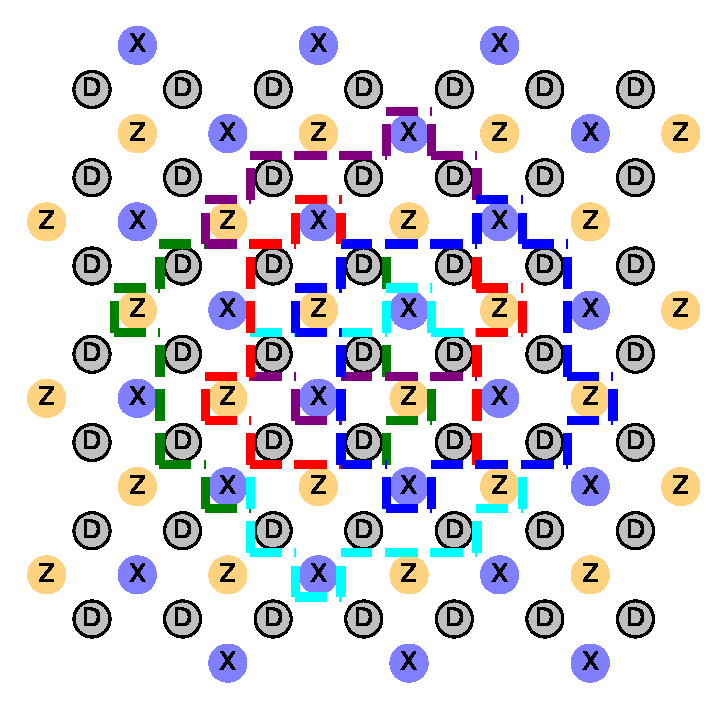
\includegraphics[width=0.6\textwidth]{d7_q25_kernels.pdf}
\ccaption
{$d=3$ kernels surrounding a data qubit in a $d=7$ surface code}
{
Illustrated in different colors are the 9 different kernel strides of the same type-4 kernel around the middle, innermost data qubit in a $d=7$ surface code. This is the only data qubit in the $d=7$ code that receives contributions from type-4 kernel strides exclusively. The kernel types, the qubit indices in each kernel, and the number of occurrences of each kernel type--kernel qubit index pair determine the number of unique contributions of kernels and contribute to the further sharing of NN weights.
}
\label{fig:d7wkern}
\end{figure*}
%%%%%%%%%%%%%%%%%%%%%%%%%%%%%

In the example shown for a $d=7$ code in Fig.~\ref{fig:d7wkern}, all of the kernels displayed in different colors are of the same type 4. 
For the simplicity of discussion in this section, we will number all data qubits from 1 (top left) to 7 (top right) and 49 (bottom right), and denote the corresponding qubit numbers on the kernel patch with a prime indicator, \eg, qubit 18 $\rightarrow$ \kernum{2} in the red kernel and \kernum{3} in the blue one, noting that the blue kernel is in flipped configuration.

The kernels displayed in the figure surround qubit 25, the only qubit that is shared exclusively by type-4 kernels alone.
We will use this qubit as an example to explain the translation of kernel outputs.
Here, the nine kernels colored in red, blue, dark green, magenta, cyan, pink, light green, brown, and orange contribute to the prediction for an error in this qubit with outputs that correspond to kernel qubit positions \kernum{5}, $\kernum{4}\equiv\kernum{6}$ (\kernum{4} in the blue kernel, but we may swap \kernum{4} and \kernum{6} due to the symmetry of type-4 kernels -- same considerations apply in magenta, pink, and light green kernels), \kernum{6}, $\kernum{8}\equiv\kernum{2}$, \kernum{2}, $\kernum{9}\equiv\kernum{1}$, $\kernum{7}\equiv\kernum{3}$, \kernum{3}, and \kernum{1} respectively. For that reason, these contributions can be encoded as a list of ordered pairs of integers as $\{(4,1)^2, (4,2)^2, (4,3)^2, (4,5), (4,6)^2\}$, with the first integer in each pair corresponding to the kernel type, the second one marking the contributing kernel qubit position, \ie, numbers with prime indicators, and the exponent indicating the number of occurrences of this pair. The number of such unique contributions ($C$) and the total count of associated parameters are listed in Table~\ref{table:unique-kern-contribs}.

%%%%%%%%%%%%%
\begin{table}[htbp]
\centering
\ccaption
{Parameter counts to combine kernels}
{
The counts are listed separately for kernel sizes $k=3$ and $k=5$ over distance-$d$ surface codes.
The numbers $C$ refer to the total number of unique combinations of kernels over all data qubits.
For any odd kernel size $k$, the values of $C$ begin to alternate with the same values for odd and even $d$ above $d=2k+1$, \ie, $d=7$ for $k=3$ and $d=11$ for $k=5$.
For smaller distances, $C=(d/2)^2$ for even and $(d^2+1)/2$ for odd $d$ values.
The composition of the unique combinations determines the number of fraction and phase parameters needed in the NN,
with the number of fractions reported for the recursive parametrization method described in the main text.
}
\renewcommand{\arraystretch}{1.25}
\begin{tabular}{c ccc ccc}
\hline
      & \multicolumn{3}{c}{$k=3$}   & \multicolumn{3}{c}{$k=5$} \\
\hline
$d$ & ~~~$C$ & Fractions & Phases & ~~~$C$ & Fractions & Phases \\
\hline
4 & ~~~4 & 5 & 8 & ~~~- & - & - \\
5 & ~~~13 & 28 & 62 & ~~~- & - & - \\
6 & ~~~9 & 27 & 80 & ~~~9 & 16 & 28 \\
7 & ~~~25 & 86 & 262 & ~~~25 & 88 & 278 \\
8 & ~~~16 & 59 & 182 & ~~~16 & 84 & 400 \\
9 & ~~~25 & 86 & 262 & ~~~41 & 268 & 1504 \\
10 & ~~~16 & 59 & 182 & ~~~25 & 194 & 1272 \\
11 & ~~~25 & 86 & 262 & ~~~61 & 522 & 3554 \\
12 & ~~~16 & 59 & 182 & ~~~36 & 328 & 2282 \\
\hline
\label{table:unique-kern-contribs}
\end{tabular}
\end{table}


If each output of a kernel were to be bounded between 0 and 1, through a sigmoid activation, and loosely be interpreted as a probability $p_i$ for an error, the combined prediction could be written through the reparametrization $x_i=\frac{p_i}{1-p_i}$. Using an analogy to write the magnitude of a complex number from a sum of two others, the parameter $x$ for the combined probability can therefore be expressed as
\begin{equation}
\begin{aligned}
Q_i &= \frac{1}{n_i}\left(\sum_{k_i=1}^{n_i} x_{k_i} + 2 \sum_{k_j=k_i+1}^{n_i} \sqrt{x_{k_i} x_{k_j}} \right), \\
S_i &= f_i Q_{i}, \\
x &= \sum_{i=1}^{N} \left( S_i + 2 \sum_{j=i+1}^{N} \sqrt{S_i S_j} c_{\varphi, ij} \right).
\end{aligned}
\label{eq:kernsum}
\end{equation}
Here, the indices $i$ and $j$ run over a total of $N$ unique kernel type--kernel qubit index pairs, \eg, $N=5$ for qubit 25, and the indices $k_i$ run over the evaluations of this unique combination $i$ in $n_i$ different strides, \eg, for the index pair $(4,5)$ of qubit 25 contributions, $k_i$ can only be 1, but it runs up to $n_i=2$ for all other index pairs.

In constructing $Q_i$, we assume that evaluations of the same combination $i$ have an underlying complex representation with the same overall phase, but $Q_i$ values with different indices $i$ do not have to carry the same phase, which justifies the phase difference parameters $c_{\varphi, ij}$.
The fractions $f_i$ are scale factors over $Q_i$ to remain agnostic on how each kernel type contributes, and are subject to the constraint $\sum_{i=1}^{N} f_i = 1$. In the implementation, they are parametrized through recursive fractions, which would satisfy the constraint by construction and avoid a spurious parameter, \ie, through the mapping $f_1 \to f_1$, $f_i \to f_i\prod_{j=1}^{i-1}\left(1-f_j\right)$ for $1<i<N$, and $f_N \to \prod_{j=1}^{N-1}\left(1-f_j\right)$. The fractions in the recursive fraction parametrization (the phase parameters $c_{\varphi, ij}$) are included as unique sets of weights between 0 (-1) and 1 that to be determined during NN training through $z$-like parameters. In order to keep their parametrization minimal, we do not include linear or quadratic dependence over $Q_i$, but this could be tested as a further expansion of the architecture in the future.

The final probability $p$, computed from the output of all kernels, could simply be found from the inverse transformation on $x$, \ie, $p=\frac{x}{1+x}$, but as a further input to the higher hierarchy of layers, we transform the final $x$ value into $z=\text{ln}(x)$ instead. Since there are $d^2$ such values, corresponding to each physical data qubit, transforming into a $z$-like variable adds more flexibility for the NN to learn nonuniform noise as one can add $d^2$ additional $z$-like trainable variables that explicitly break any symmetries.
